\chapter{Spatially Random Maps}
As studying the effects of random spatial perturbations
on the dynamics of one-dimensional maps may yield implications for
understanding the dynamics on higher dimensional maps, we present two
case studies:
\begin{enumerate}
\item the logistic map,
\item the circle map.
\end{enumerate}
The random spatial perturbations in both maps are intended to mimic
the noise used in hydraulic modeling for the porosity and hydraulic
conductivity, which is assumed to be log-normal with an
exponentially decaying spatial correlation. Observations
in subsurface hydrology suggest flow parameters are
log-normal~\cite{gelhar}. The following sections offer background
information on the nature of the spatially random processes and the characteristics of both maps with the spatial perturbations. 
\section{Spatially Random Processes}\label{spatprocs}
The noise in hydraulic modeling is often assumed to be log-normal with an
exponentially decaying spatial correlation, so we let
\begin{equation}\label{R}
\xi(x)=\ln(R(x)) 
\end{equation}
be a normal random variable~\cite{gelhar} that represents the noise. Then
$R(x)$ is a log-normal random variable. A normal distribution may be used
for subsurface storage properties\footnote{Some examples of subsurface
storage properties include porosity and moisture content.}, but in some cases, it is
inappropriate because it would imply negative values have nonzero
probability. Alternatively, a log-normal random variable may
be used for physical parameters known to be nonnegative. Moreover, the log-normal distribution frequently appears when observing
nonnegative flow parameters underground, like hydraulic conductivity and
transmissivity~\cite{gelhar}. An important property we would like to
capture in this process is how the noise should vary based on
position. In aquifers, porosity in a neighborhood of rock tends to be
somewhat consistent (highly correlated), whereas porosity between two
areas on opposite ends of the aquifer can be completely
different. Thus, the noise in the random process should depend on the
distance between two locations instead of the locations themselves,
and we call this property homogeneity. 

We begin to characterize the process by
assuming the entire random process $\xi(x)$ is homogeneous, and defining the mean $\mu$ and variance $\sigma^2$
of $\xi(x)$ to be
\begin{align}
\begin{split}\label{ximean}
\mu &= E[\xi(x)] = \ln(r)\\
\sigma^2 &= E[(\xi(x) - \mu)^2]=E[\xi(x)^2]-(\ln(r))^2.
\end{split}
\end{align}
From probability, the definition of covariance is~\cite{ross}
\begin{align*}
\begin{split}
C(x,y) &= E[(x - E[x])(y - E[y])]\\
&= E[xy] - E[x]E[y].
\end{split}
\end{align*}
Let us compute $C(y+x,y)$,
\begin{align*}
\begin{split}
C(y+x,y) &= E[(y+x - E[y+x])(y - E[y])]\\
&= E[ (y+x)y - (y+x)E[y] -yE[y+x] + E[y+x]E[y] ]\\
%&= E[y^2 + xy] - E[y+x]E[y] - E[y]E[y+x] + E[y+x]E[y]\\
&= E[y^2 + xy] - E[y+x]E[y] \\
&= E[y^2] - (E[y])^2 + E[xy] - E[x]E[y]\\
&= Var(y) + Cov(x,y).
\end{split}
\end{align*}
As the entire process is homogeneous, the covariance is also
homogeneous. Indeed, if the covariance function is defined as a function of $x,y$, but the
variability is independent of location in space; rather, dependent on
the separation vector between the locations, we call the covariance
function homogeneous~\cite{gelhar}. Thus, covariance is
\begin{align}
\begin{split}\label{cor}
C(x) &= E[(\xi(x+y) - E[\xi(x)])(\xi(y)-E[\xi(x)])] \\
&= E[(\xi(x+y) -\ln(r))(\xi(y)-\ln(r))]. 
\end{split}
\end{align}
The noise in nonnegative flow parameters is
thought to rely on the distance between two points instead of their
precise locations, so $C(x)$ in (\ref{cor}) is
homogeneous. $C(x)$ is also called a correlation function, which
describes how variables at different positions in space are
related. It physically represents the degree of correlation between
two consecutive instances in the process. Correlations are strongest
when iterates are nearby, and they typically decay as the distance
between two iterates increases, although random processes could violate this assumption. 

We construct a random function $\xi(x)$ on $[0,1]$ that satisfies
(\ref{ximean}) with an infinite Fourier Series,
\begin{align}\label{fs1}
\xi(x) = \ln(r) + \sum_{n \in \mathbb{Z}}\hat{\xi_n}e^{2\pi inx}.
\end{align}
Desirably, the magnitudes of the Fourier modes $\hat{\xi_n}$ diminish
as $n \to \pm \infty$, which implies the random log-fluctuations are
not identically distributed. To ensure~(\ref{fs1}) stays in the real plane, we impose the condition
\begin{align}\label{realcond}
\hat{\xi}_{n}^* = \hat{\xi}_{-n},
\end{align}
where $\hat{\xi}_n=a_n + ib_n \in \mathbb{C}$ and the $*$ operator denotes the complex conjugate. Equation (\ref{fs1}) assumes $a_0=0$
because we wish to maintain $E[\xi(x)]=\ln(r)$ when $n=0$ (the
spatially independent term $a_0$ will be absorbed into $\ln(r)$).
Since the expectation of a sum is equal to the sum of
expectations, we find~\cite{ross}
\begin{align*}
\begin{split}
E[\xi(x)] &= E[\ln(r) + \sum_{n \in \mathbb{Z}}\hat{\xi_n}e^{2\pi
  inx}]\\
&= \ln(r) + E[\sum_{n \in \mathbb{Z}}\hat{\xi_n}e^{2\pi inx}]\\
&= \ln(r) + \sum_{n \in \mathbb{Z}}e^{2\pi inx}E[\hat{\xi_n}].
\end{split}
\end{align*}
If we choose the mean of the
magnitude of the Fourier modes $|\hat{\xi}_n|$ to be zero, then the mean of the Fourier
Series is zero, which preserves the expected value of $\xi(x)$ in~(\ref{ximean}). Therefore, we let
\begin{align}
\begin{split}\label{xihatmean}
\hat{\mu}_n&=E[|\hat{\xi}_n|]=0\\
\hat{\sigma}_n^2&=E[|\hat{\xi}_n|^2]-(E[|\hat{\xi}_n|])^2=E[|\hat{\xi}_n|^2].
\end{split}
\end{align}
For notation, let the function $S:\mathbb{Z} \to \mathbb{R}$ be
\begin{equation}\label{Sn}
S(n) = \hat{\sigma}_n^2.
\end{equation}
Equation~(\ref{Sn}) is also called the spectral density function. If we
assume the modes $|\hat{\xi}_n|$ are independent, then the product of
two modes $n,m$, where $m \neq -n$, have expectation
\begin{align*}
\begin{split}
E[|\hat{\xi}_n||\hat{\xi}_m|]&=E[|\hat{\xi}_n|]E[|\hat{\xi}_m|]\\
&=0.
\end{split}
\end{align*}
However, if $m=-n$, 
\begin{align*}
\begin{split}
E[|\hat{\xi}_n||\hat{\xi}_{-n}|]&= E[\hat{\xi}_n\hat{\xi}_n^*]\\
&=E[a_n^2+b_n^2]\\
&=E[|\hat{\xi}_n|^2]
\end{split}
\end{align*}
which follows from~(\ref{realcond}). In other words,
\begin{displaymath}
E[|\hat{\xi}_n||\hat{\xi}_m|] = \left\{
     \begin{array}{lr}
       S(n) & : m = -n\\
       0 & : m \neq -n.\\
     \end{array}
   \right.
\end{displaymath} 
We introduce the notion of the spectral density function $S(n)$ as the Fourier transform
of the correlation function~(\ref{cor})~\cite{gelhar}.
\begin{align}
\begin{split}\label{homog}
\hat{C}(k) &= \int_{0}^{1}C(x)e^{-2\pi ikx}dx\\
&= \sum_{m,n} \int_{0}^{1} E[|\hat{\xi}_n||\hat{\xi}_m|] e^{2\pi
  im(x+y)}e^{2\pi iny}e^{-2\pi ikx}dx\\
&=S(k).
\end{split}
\end{align}
Equation~(\ref{homog}) is homogeneous, so this implies $(a_n,b_n)$ are
independent. By nature of being defined as the Fourier transform of
the covariance function, the spectrum represents a distribution of variance over
frequency. In fact, for $x=0$, (\ref{cor}) reduces to the definition
of variance of $\xi(x)$, so 
\begin{align*}
\begin{split}
C(x) &= \sum_{n\in \mathbb{Z}}S(n)e^{2\pi inx}\\
C(0) &= \sigma^2 = \sum_{n\in \mathbb{Z}}S(n).
\end{split}
\end{align*}
A simple spectrum that falls off quickly is
\begin{align}\label{spec}
S(n)=\alpha e^{-L|n|},
\end{align}
where $L \in [0,1]$ is the correlation length (and is fixed
for each simulation). Values of $L$ close to zero will result in a
small, negative exponent, which consequently increases the
spectrum. On the other hand, larger values of $L$ cause
the spectrum to decay faster. This choice of $S(n)$ corresponds to a correlation function
\begin{align*}
\begin{split}
C(x) &= \sum_{n\in \mathbb{Z}}S(n)e^{2\pi inx}=\sum_{n\in \mathbb{Z}}\alpha \frac{1}{e^{L|n|}}e^{2\pi inx}\\
&= \alpha + \sum_{n=1}^{\infty}\alpha e^{2\pi
  inx-L|n|}+\sum_{n=-1}^{-\infty}\alpha e^{2\pi inx-L|n|}\\
&= \alpha+\alpha \sum_{n=1}^{\infty}(e^{2\pi ix-L})^n+\alpha \sum_{m=1}^{\infty}(e^{-2\pi ix-L})^m\\
&=\alpha + \alpha \frac{e^{2\pi ix-L}}{1-e^{2\pi ix-L}} +\alpha
\frac{e^{-2\pi ix-L}}{1-e^{-2\pi ix-L}}\\
&=\alpha \left(1+ \frac{-2e^{-2L}+2\cos(2\pi x)e^{-L}}{e^{-2L}-2\cos(2\pi x)e^{-L}+1} \right).\\
\end{split}
\end{align*}
Finally,
\begin{align}\label{cx}
C(x)= \alpha \frac{e^{2L}-1}{e^{2L}-2\cos(2\pi x)e^L+1}.
\end{align}
Figure~\ref{fig:covspec} demonstrates an example of a covariance-spectrum
pair from~(\ref{cx}) and~(\ref{spec}). In~(\ref{spec}) and~(\ref{cx}), the parameter $\alpha$ is a constant used to normalize
$C(x)$.
\begin{figure}[htp]
\caption[Schematic example of the covariance-spectrum pair]{The correlation function
  $C(x)$ and the spectral density $S(n)$ for $L=0.5,\sigma=0.0216, \alpha=0.000114$.}\label{fig:covspec}
\centering
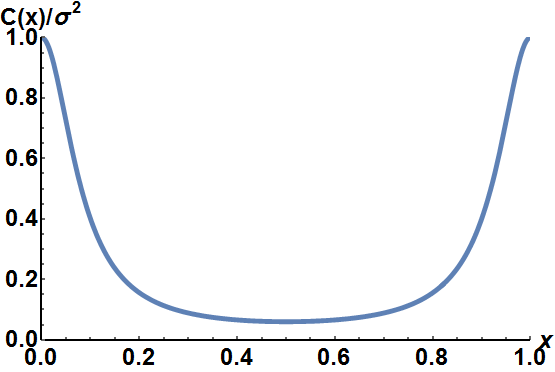
\includegraphics[width=.45\textwidth]{figs/cx.png}\hfill
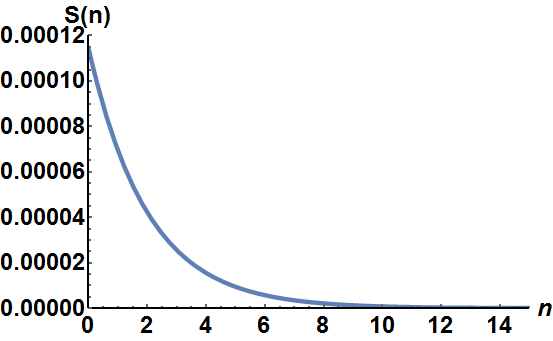
\includegraphics[width=.45\textwidth]{figs/sn.png}
\end{figure}
Recall from~(\ref{cor}) when $x=0$, the covariance function reduces to the definition
of variance, therefore
\begin{align}
\begin{split}\label{a}
\sigma^2&= \alpha \frac{e^{2L}-1}{e^{2L}-2\cos(0)e^L+1}\\
\alpha &=\sigma^2 \frac{e^{2L}-2e^{L} +1}{e^{2L}-1}\\
\alpha &=\sigma^2
\frac{(e^{L}-1)^2}{(e^{L}-1)(e^{L}+1)}\\
\alpha &= \sigma^2 \tanh(L/2).
\end{split}
\end{align}
The parameter $\alpha$ is now defined in terms of the variance
$\sigma^2$ of $\xi(x)$. Examples of the function $C(x)$ are demonstrated in Figure~\ref{fig:correlation}
for various values of $L$.
\begin{figure}[htp]
\caption[The correlation function $C(x)$]{The correlation function
  $C(x)$ for $L \in \{0.1,0.5,1\}$. For small $L$
  (leftmost graph), the correlation is stronger between iterates than for large $L$
  (rightmost graph).}\label{fig:correlation}
\centering
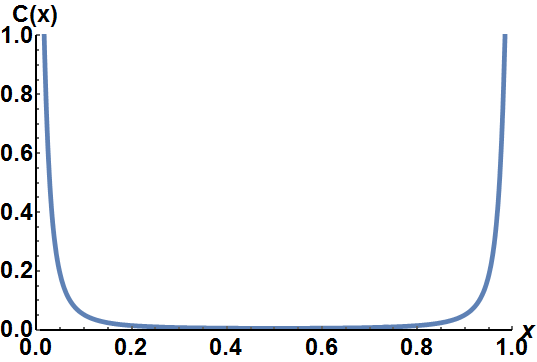
\includegraphics[width=.3\textwidth]{figs/correlation_L01.png}\hfill
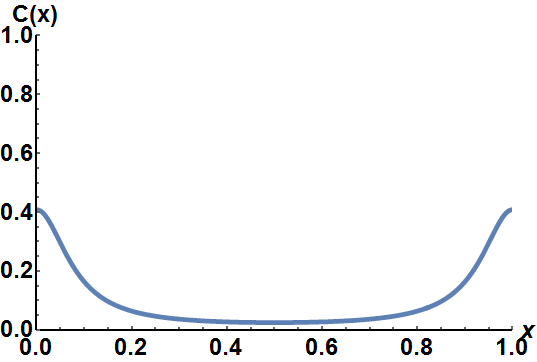
\includegraphics[width=.3\textwidth]{figs/correlation_L05.png}\hfill
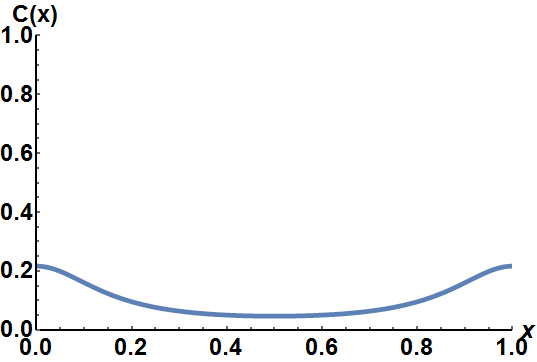
\includegraphics[width=.3\textwidth]{figs/correlation_L1.png}
\end{figure}

We may wish to bound the distribution of the noise, especially if we
apply the noise to the logistic map. Its parameter $r$ must take on
values in the interval $[0,4]$, or else iterates of the map may leave $[0,1]$. If we
substitute the constant parameter $r$ for $R(x)$, we require
$R(x) \leq 4$. One way to prevent the possibility of exiting $[0,1]$ is to bound the distribution of $\hat{\xi}_n$ from~(\ref{fs1}). Suppose the probability density
function for $\hat{\xi}_n$ is nonzero only in the complex square centered at the
origin with side length $2M_n$ (shown in Figure~\ref{fig:square}). Thus, $|a_n|,|b_n| \leq M_n$, and for a fixed $r$, we
can bound $\ln(R(x))$ using~(\ref{R}) and~(\ref{fs1}). First, recall
\begin{align*}
\xi(x) = \ln(R(x)),
\end{align*}
and because we want $R(x) \leq 4$, this implies
\begin{align*}
\xi(x) = \ln(R(x)) \leq \ln(4).
\end{align*}
Since we also defined $\xi(x)$ as a series, we have
\begin{align*}
\xi(x) =\ln(R(x))= \ln(r) + \sum_{n \in \mathbb{Z}}\hat{\xi_n}e^{2\pi inx} \leq \ln(r) + \sum_{n \in \mathbb{Z}}|\hat{\xi_n}|,
\end{align*}
where $r$ is fixed for any given realization. If the sum over the magnitude of the Fourier modes is bounded by a constant, $\xi(x)$ will also be bounded by the same limit; therefore we choose
\begin{align*}
\begin{split}
\ln(r) + \sum_{n \in \mathbb{Z}}|\hat{\xi_n}| &\leq \ln(4)\\
\sum_{n \in \mathbb{Z}}|\hat{\xi_n}| &\leq \ln(4/r).
\end{split}
\end{align*}
We have $|\hat{\xi_n}| = \sqrt{a_n^2 + b_n^2}$ and $|a_n|,|b_n| \leq M_n$, which implies
\begin{align}
\begin{split}\label{bdnr}
\sum_{n \in \mathbb{Z}}|\hat{\xi_n}| =\sum_{n \in \mathbb{Z}}\sqrt{a_n^2 + b_n^2} &\leq \sum_{n \in
  \mathbb{Z}}|a_n| + |b_n|\\
&\leq \sum_{n \in \mathbb{Z}}2M_n\\
&\leq \ln(4/r).
\end{split}
\end{align}
What remains is to choose $M_n$ such that the sum in~(\ref{bdnr}) is
bounded by $\ln(4/r)$. In order for this to occur, the sequence of side lengths $M_n$ must be summable. 
\begin{figure}[!h]
\caption[Uniform Distribution over a Square Region]{The probability
  density function of $\hat{\xi_n}$ is uniformly distributed across
  this square region, centered at the origin. The square region has
  side length $2M_n$ and area $4M_n^2$.}\label{fig:square}
	\begin{center}
		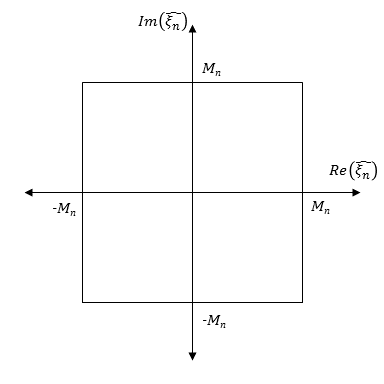
\includegraphics[scale=0.7]{figs/square.png}
	\end{center}
\end{figure}

Let $\hat{\xi}_n$ be uniformly distributed, so 
\begin{equation}\label{eq:square}
   h(\hat{\xi}_n) =h(a,b)= \left\{
     \begin{array}{lr}
       \frac{1}{4 M_n^2} & |a_n|,|b_n| \leq M_n\\
       0 & |a_n|,|b_n| > M_n\\
     \end{array}
   \right.
\end{equation} 
where $h:\mathbb{C}\to [0,1]\in \mathbb{R}$ is the probability density
function of $\hat{\xi}_n$. To find the relationship between $S(n)$ and
$M_n$, recall that $S(n)$ is defined as the variance of the
log-fluctuations~(\ref{Sn}). Then, 
\begin{align}
\begin{split}\label{Mn}
S(n)&=E[|\hat{\xi}_n|^2] = E[a^2+b^2]\\
 &= \frac{1}{4M_n^2}\int_{-M_n}^{M_n}\int_{-M_n}^{M_n}(a^2+b^2)\,da\,db\\
&=\frac{2}{3}M_n^2\\
M_n&=\sqrt{\frac{3}{2}S(n)}.
\end{split}
\end{align}
Finally, using the expression for $\alpha$~(\ref{a}), the
expression for $M_n$~(\ref{Mn}), and the sum from~(\ref{bdnr}), let
\begin{align*}
A = M_0+2\sum_{n=1}^\infty M_n \leq \ln(4/r).
\end{align*}
Then, we find
\begin{align*}
\begin{split}
A &=\left(\sqrt{\frac{3}{2}\alpha} +
2\sqrt{\frac{3}{2}\alpha}\sum_{n=1}^{\infty}e^{-Ln/2}\right) \\
&= \sqrt{\frac{3}{2}}\alpha\left(1+ \frac{2e^{-L/2}}{1-e^{-L/2}} \right)\\
&= \sigma\sqrt{\frac{3}{2}}
\sqrt{\tanh(L/2)}\left(\frac{e^{L/2}+1}{e^{L/2}-1} \right)\\
&= \sigma \sqrt{\frac{3}{2}}\frac{\sqrt{\tanh(L/2)}}{\tanh(L/4)} \leq \ln(4/r).\\
\end{split}
\end{align*}
Thus, the standard deviation $\sigma$ must be bounded from below by
zero and from above by
\begin{align}\label{sigma}
0<\sigma \leq \ln(4/r)\sqrt{\frac{2}{3}}\frac{\tanh(L/4)}{\sqrt{\tanh(L/2)}}.
\end{align}
Figure~\ref{fig:R} is a sample realization of a function $R(x)$ that
behaves according to~(\ref{sigma}).
\begin{figure}[!h]
\caption[The function $R(x)$]{The function $R:[0,1]\to [0,4]$ where
  $\sigma=0.0386, L=0.1, r=3.5, N=100$}\label{fig:R}
	\begin{center}
		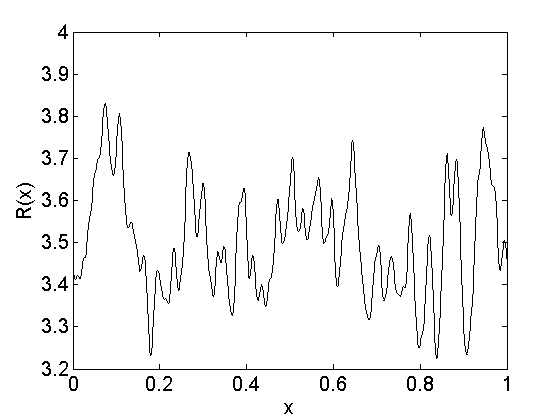
\includegraphics[scale=0.6]{figs/xi.png}
	\end{center}
\end{figure}

An application of the Lyapunov Central
Limit Theorem demonstrates that the sum over independent, non-identical uniform
random variables $\hat{\xi}_n$ tends to the normal distribution~\cite{billingsley}.

\begin{singlespacing}
\begin{theorem}\label{clt}
Let $\hat{\xi}_1, \hat{\xi}_2, ...\hat{\xi}_m$ be a sequence of independently distributed random
variables, each having mean $E[\hat{\xi}_n]=\hat{\mu}_n$ and variance
$\hat{\sigma}_n^2 < \infty$. Define
\begin{align*}
\begin{split}
Y_n &=\hat{\xi}_n - \hat{\mu}_n\\
T_m &= \sum_{n=1}^{m}Y_n\\
s_m^2 &=\sum_{n=1}^m\hat{\sigma}_n^2.
\end{split}
\end{align*}
if $\exists\, \delta>0$ such that 
\begin{align*}
\lim_{m\to \infty}\frac{1}{s_m^{2+\delta}}\sum_{n=1}^mE[|Y_n|^{2+\delta}] \to 0,
\end{align*}
then the distribution of
\begin{equation*}
\frac{T_m}{s_m} \sim N(0,1).
\end{equation*}
That is, $\frac{T_m}{s_m}$ tends to the standard normal.
\end{theorem}
\end{singlespacing}

Based on the definitions in Theorem~\ref{clt}, we have for
$|\hat{\xi}_n| \sim Unif(-M_n,M_n)$
\begin{align*}
\begin{split}
Y_n &= |\hat{\xi}_n| - \hat{\mu}_n = |\hat{\xi}_n|\\
T_m &= |\hat{\xi}_{-m}|+|\hat{\xi}_{-m+1}|+ ...+|\hat{\xi}_{0}|+|\hat{\xi}_{1}|+...+|\hat{\xi}_{m}|\\
&=
|\hat{\xi}_{1}|+|\hat{\xi}_{1}^*|+...+|\hat{\xi}_{m}|+|\hat{\xi}_{m}^*|\\
&= \sum_{n=1}^{m} 2|\hat{\xi}_{n}|,
\end{split}
\end{align*}
since $\hat{\xi}_{0} = 0$. A uniform random variable $X\sim Unif(a,b)$ has variance
$Var(X) = \frac{1}{12}(b-a)^2$, so
\begin{align*}
\begin{split}
\hat{\sigma}_n^2 &= \frac{1}{3}M_n^2\\
&= \frac{1}{3}\frac{3}{2}S(n)\\
&= \frac{1}{2}\alpha e^{-L|n|}\\
s_m^2 &= \frac{\alpha}{2}\left(e^{-L|-m|}+e^{-L|-m+1|}+...+1+e^{-L}+...e^{-Lm} \right)\\
&= \frac{\alpha}{2} + \alpha \left(e^{-L}+...e^{-Lm} \right)\\
&=\frac{\alpha}{2} +\alpha\sum_{n=1}^m e^{-Ln}.
\end{split}
\end{align*}
We check whether the sum $s_m^2$ diverges as $m \to \infty$. After applying the Geometric series identity,
\begin{align*}
\begin{split}
s_m^2 &=\frac{\alpha}{2} +\alpha\sum_{n=1}^\infty e^{-Ln}\\
&= \frac{\alpha}{2} + \left( \frac{\alpha}{1-e^{-L}}- \alpha\right)\\
&= \frac{\alpha(e^L+1)}{2(e^L-1)}\\
&= \frac{\alpha}{2 \tanh(L/2)}.
\end{split}
\end{align*}
It is convenient to calculate the moments of a random variable $X$ as a
way of finding $E[X^n]$. The $k$th moment of a uniform random variable $X \sim
Unif(a,b)$ is defined as 
\begin{align*}
m_k = \frac{1}{k+1}\sum_{i=0}^ka^ib^{k-i}.
\end{align*}
If we choose $\delta=1$, then 
\begin{align*}
\begin{split}
\lim_{m \to \infty}s_m^3&=\left(\frac{\alpha}{2 \tanh(L/2)}\right)^{3/2}\\
E[|\hat{\xi}_{n}|^3] &=\frac{1}{4} (-M_n + M_n)4M_n^2 = 0.
\end{split}
\end{align*}
Therefore, 
\begin{align*}
\begin{split}
\lim_{m\to
  \infty}\frac{1}{s_m^{2+\delta}}\sum_{n=1}^mE[|Y_n|^{2+\delta}] &= \lim_{m\to
  \infty}\frac{1}{s_m^{3}}\lim_{m\to
  \infty}\sum_{n=1}^mE[|\hat{\xi}_{n}|^{3}] \\
&= \left(\frac{\alpha}{2 \tanh(L/2)}\right)^{-3/2}\lim_{m\to \infty}\sum_{n=1}^m 0 \\
&= 0.
\end{split}
\end{align*}
Thus, 
\begin{align*}
\frac{T_m}{s_m} = \frac{2}{\sqrt{\frac{\alpha}{2} +\alpha\sum_{n=1}^m e^{-Ln}}} \sum_{n=1}^{m} |\hat{\xi}_{n}|\sim N(0,1),
\end{align*}
which implies the transformation $\xi(x)$ of this sum is also normal,
as desired.  

In summary, for each realization of the random process, the noise
$\xi(x)$ is normally distributed, which implies $R(x)$ is a log-normal
random variable. The Fourier modes of $\xi(x)$ are uniform random variables $a_n,b_n \sim Unif(-M_n,M_n)$ whose bounds are set by
$M_n= \sqrt{\frac{3}{2}S(n)}$, where $S(n)=\alpha e^{-L|n|}$, the
spectral density, was chosen to decay exponentially fast. The constant $\alpha = \sigma^2 \tanh(L/2)$ normalizes the corresponding
correlation function $C(x)$, where the standard deviation $\sigma$ of
the noise $\xi(x)$
must be bound according to~(\ref{sigma}) in order to restrict $R(x)$
to $[0,4]$ to ensure $[0,1]$ is an invariant set of
$f$.

\section{Random Dynamics of the Logistic Map}
The spatially random logistic map has not been as well explored in the
literature as the temporally random case~\cite{athreya}. Athreya and
Dai explore the concept of a time-varying logistic map, where the
parameter $r_i$ is a function of each time step, as opposed to position
in space. At each time step, some $r_i \in \{r\}_0^\infty$ is applied
to the map, where the
sequence $\{r\}_0^\infty$ has independent and identically distributed
random variables in [0,4]. In contrast, the spatially random logistic
map replaces the parameter $r$ from~(\ref{logmap}) with a random
function of space, $R:[0,1]\to [0,4]$. In line with the deterministic map, 
$f:[0,1]\to [0,1]$, where
\begin{equation}\label{randlogmap}
x_{n+1} = f(x_n) = R(x_n)x_n(1-x_n).
\end{equation}
Numerical simulations of~(\ref{randlogmap}) require a discrete limit
on the sum in~(\ref{fs1}). We can combine
the equations in~(\ref{fs1}) and~(\ref{realcond}) to arrive at the following form for
$\xi(x)$,
\begin{align}\label{fs2}
\xi(x) = \ln(r) + 2\sum^N_{n=1}a_n\cos(2\pi nx)-b_n\sin(2\pi nx),
\end{align}
where $N$ represents the number of Fourier modes in the sum, and is an
upper limit that we impose on the summation\footnote{In practice, $N
  \approx 10/L$, where $L$ represents the correlation length. $N$
  should be chosen to be large enough such that the Fourier amplitudes
may decay as more terms are included. This restriction will ensure the
fluctuations are log-normal.}. Figure~\ref{fig:rlogstable} demonstrates one realization of a spatially random logistic map.
\begin{figure}[!h]
\caption[Random logistic map, stable orbit]{One instance of a random
  logistic map (blue), which was iterated for 1000 steps. The map has converged to a stable period 4 orbit (green). Notice the
  ``wiggliness'' in the parabola shape. $r=3.5,L=0.05,N=200,\sigma=0.0061$}\label{fig:rlogstable}
	\begin{center}
		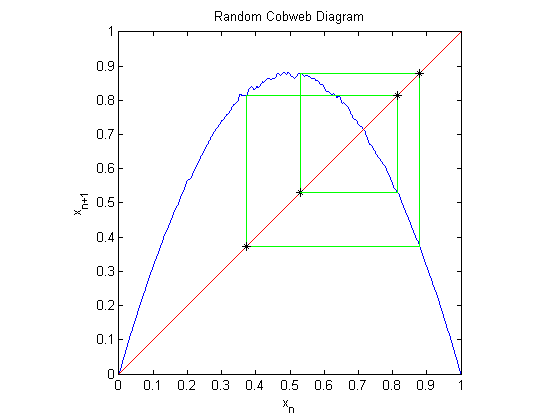
\includegraphics[scale=0.7]{figs/rand_cobweb.png}
	\end{center}
\end{figure}
 Figure~\ref{fig:envelope} depicts rough estimates\footnote{The
  maxima and minima over 500 samples were recorded and plotted in
  these figures.} of upper and lower bounds for the random logistic
map for various sets of parameters. 
\begin{figure}[htp]
\caption[Upper and lower bounds on the random logistic map]{A coarse
  demonstration (500 samples) of the upper and lower bounds of the random logistic
  map. Sample realizations are shown in red. From left to right:
  $\{\sigma=0.1093,r=2.7,L=0.9,N=112\}, \{\sigma=0.0086,r=3.5,L=0.05,N=200\},\{\sigma=0.0071,r=3.7,L=0.1,N=100\}$
  }\label{fig:envelope}
\centering
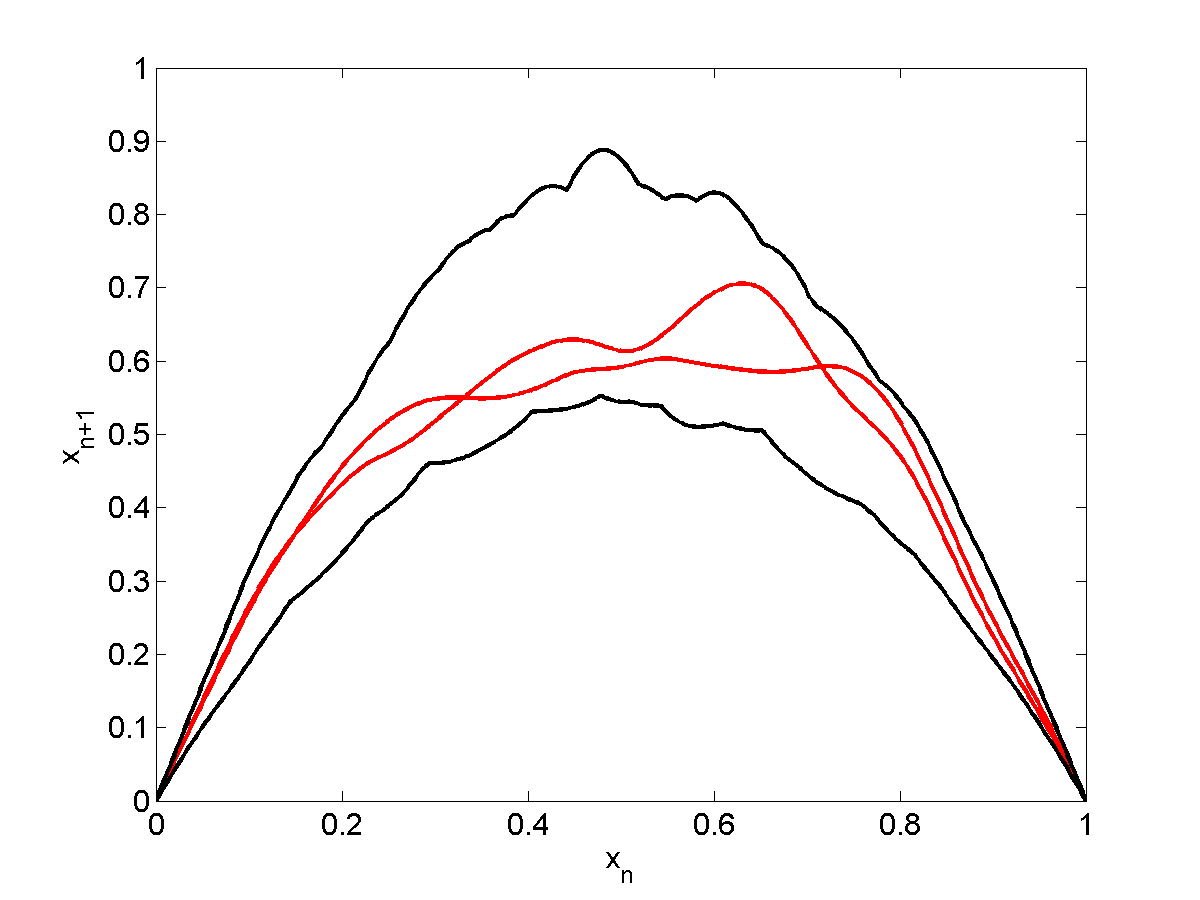
\includegraphics[width=.3\textwidth]{figs/envelope_500_r27_L09.png}\hfill
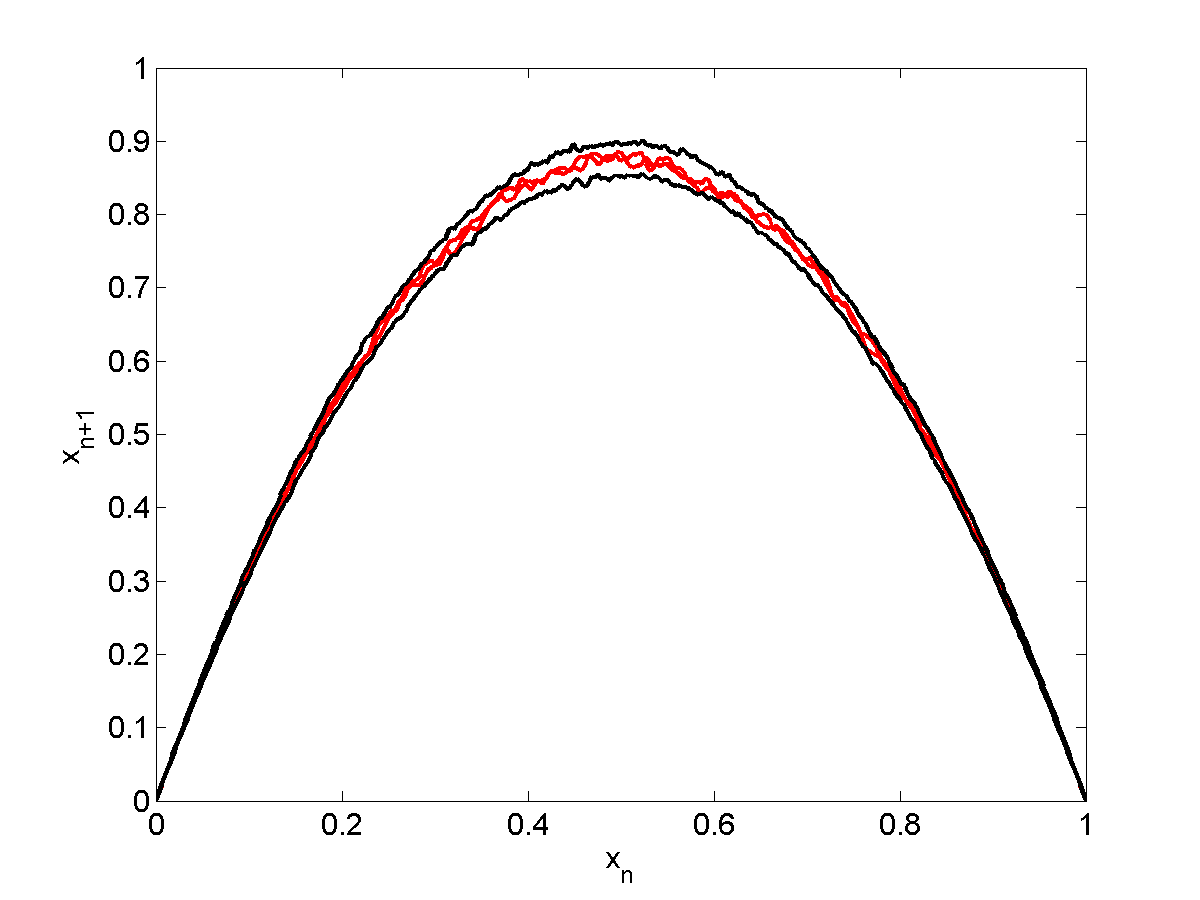
\includegraphics[width=.3\textwidth]{figs/envelope_500_r35_L005.png}\hfill
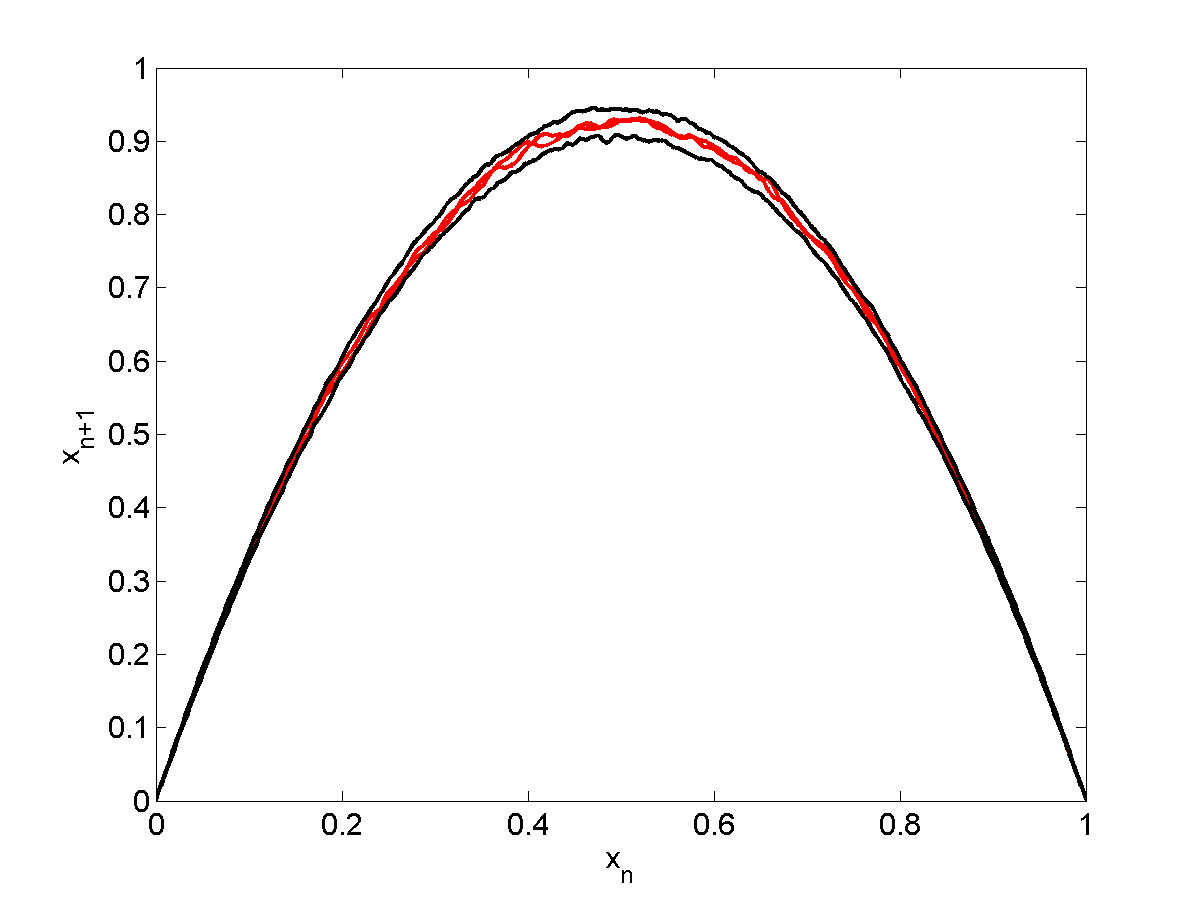
\includegraphics[width=.3\textwidth]{figs/envelope_500_r37_L01.png}
\end{figure}

\section{Random Dynamics of the Circle Map}
We will investigate a spatially random circle map of the form
\begin{align}\label{randcirc}
x_{n+1}= F(x_n) =  x_n + \Omega(x_n) - \frac{k}{2\pi}\sin(2\pi x_n),
\end{align}
where $\omega$ from~(\ref{detcirc}) has been replaced with a function
of space, $\Omega:S^1\to S^1$. To distinguish between the logistic map
and the circle map, we denote the function $R(x)$ in~(\ref{R}) as
$\Omega(x)$; that is, $\Omega(x)$ is also a log-normal random variable
and has the same properties as $R(x)$ from Section~\ref{spatprocs}. In Figure~\ref{fig:rcircstable}, a realization of the
random circle map using the probability density function $h$ from~(\ref{eq:square}) is shown,
where the orbit converges to a period 5 orbit. 
\begin{figure}[!h]
\caption[Random circle map, stable orbit]{The cobweb
  diagram (green) for a random realization of the circle map (blue) with $\omega =
  0.3, k=1, \alpha = 10^{-5}$. The line $x_{n+1}=x_n$ is drawn in red. The orbit
  has converged to a stable period 5 orbit. Its basin of attraction is
  $S^1$. Transient iterations were removed.}\label{fig:rcircstable}
	\begin{center}
		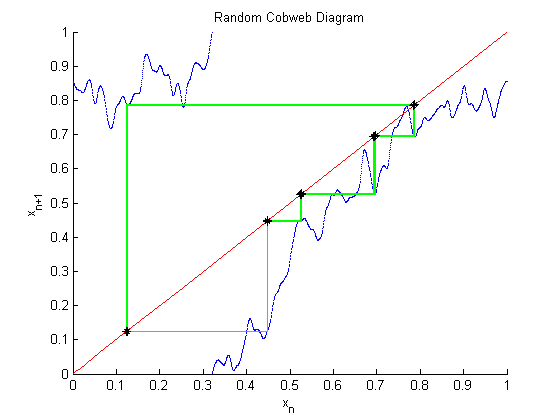
\includegraphics[scale=0.7]{figs/randcirc_cobweb.png}
	\end{center}
\end{figure}
Numerical simulations of~(\ref{randcirc}) require a finite number of
terms in the Fourier series of $\xi(x)$ in~(\ref{fs1}). Therefore, we find
\begin{align}\label{fs_circ}
\xi(x) = \ln(\omega) + 2\sum^N_{n=1}a_n\cos(2\pi nx)-b_n\sin(2\pi nx).
\end{align}
However, since we
do not require $\Omega(x)$ of the circle map~(\ref{randcirc}) to be bounded as strictly
as $R(x)$ of the logistic map~(\ref{randlogmap}), $\alpha$ may be
chosen freely, and $h(a,b)$ is not limited to the bounded uniform
distribution. The choice of $h(a,b)$ should fulfill the conditions of
the Lyapunov Central Limit Theorem (Theorem~\ref{clt}) in order to
guarantee the noise is log-normal.

Overall, we have a much simpler set of equations for the circle map
than for the logistic map since $\Omega(x)$ is unrestricted. For each realization of the map, we choose
a set of random variables $a_n, b_n$ that correspond to the Fourier
modes of $\xi(x)$, and may be drawn from an
unbounded distribution, as long as the variance decays according to
the spectral density $S(n)$ in~(\ref{Sn}). 